% Created by tikzDevice version 0.10.1 on 2018-02-18 23:12:18
% !TEX encoding = UTF-8 Unicode
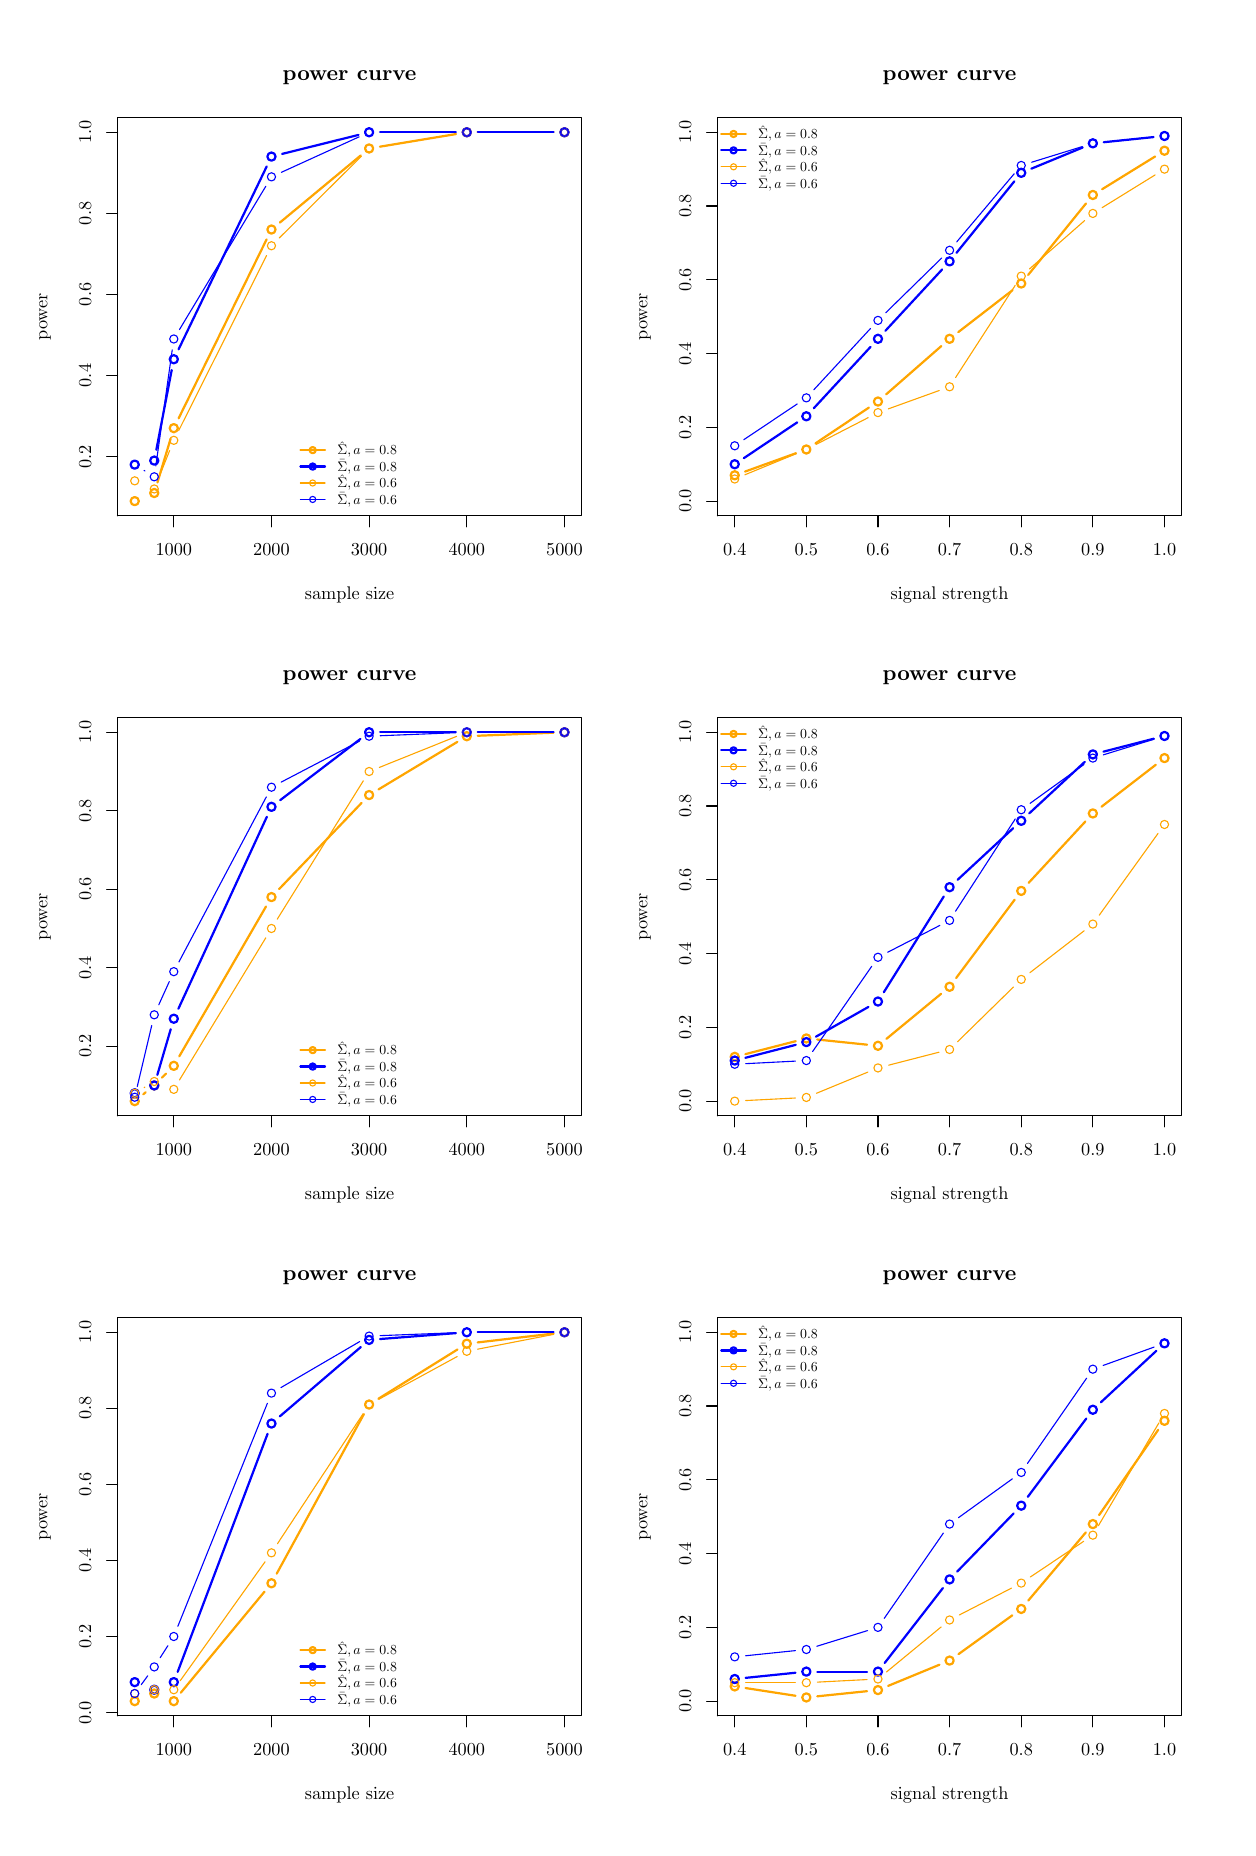
\begin{tikzpicture}[x=1pt,y=1pt]
\definecolor{fillColor}{RGB}{255,255,255}
\path[use as bounding box,fill=fillColor,fill opacity=0.00] (0,0) rectangle (433.62,650.43);
\begin{scope}
\path[clip] ( 32.47,474.01) rectangle (200.18,617.96);
\definecolor{drawColor}{RGB}{255,165,0}

\path[draw=drawColor,line width= 0.8pt,line join=round,line cap=round] ( 46.88,486.06) -- ( 51.66,501.92);

\path[draw=drawColor,line width= 0.8pt,line join=round,line cap=round] ( 54.55,509.26) -- ( 86.34,573.92);

\path[draw=drawColor,line width= 0.8pt,line join=round,line cap=round] ( 91.14,580.00) -- (120.34,604.24);

\path[draw=drawColor,line width= 0.8pt,line join=round,line cap=round] (127.29,607.42) -- (154.77,611.98);

\path[draw=drawColor,line width= 0.8pt,line join=round,line cap=round] (162.64,612.63) -- (190.01,612.63);

\path[draw=drawColor,line width= 0.8pt,line join=round,line cap=round] ( 38.68,479.34) circle (  1.48);

\path[draw=drawColor,line width= 0.8pt,line join=round,line cap=round] ( 45.74,482.27) circle (  1.48);

\path[draw=drawColor,line width= 0.8pt,line join=round,line cap=round] ( 52.80,505.71) circle (  1.48);

\path[draw=drawColor,line width= 0.8pt,line join=round,line cap=round] ( 88.09,577.48) circle (  1.48);

\path[draw=drawColor,line width= 0.8pt,line join=round,line cap=round] (123.38,606.77) circle (  1.48);

\path[draw=drawColor,line width= 0.8pt,line join=round,line cap=round] (158.67,612.63) circle (  1.48);

\path[draw=drawColor,line width= 0.8pt,line join=round,line cap=round] (193.97,612.63) circle (  1.48);
\end{scope}
\begin{scope}
\path[clip] (  0.00,  0.00) rectangle (433.62,650.43);
\definecolor{drawColor}{RGB}{0,0,0}

\path[draw=drawColor,line width= 0.4pt,line join=round,line cap=round] ( 52.80,474.01) -- (193.97,474.01);

\path[draw=drawColor,line width= 0.4pt,line join=round,line cap=round] ( 52.80,474.01) -- ( 52.80,470.05);

\path[draw=drawColor,line width= 0.4pt,line join=round,line cap=round] ( 88.09,474.01) -- ( 88.09,470.05);

\path[draw=drawColor,line width= 0.4pt,line join=round,line cap=round] (123.38,474.01) -- (123.38,470.05);

\path[draw=drawColor,line width= 0.4pt,line join=round,line cap=round] (158.67,474.01) -- (158.67,470.05);

\path[draw=drawColor,line width= 0.4pt,line join=round,line cap=round] (193.97,474.01) -- (193.97,470.05);

\node[text=drawColor,anchor=base,inner sep=0pt, outer sep=0pt, scale=  0.66] at ( 52.80,459.76) {1000};

\node[text=drawColor,anchor=base,inner sep=0pt, outer sep=0pt, scale=  0.66] at ( 88.09,459.76) {2000};

\node[text=drawColor,anchor=base,inner sep=0pt, outer sep=0pt, scale=  0.66] at (123.38,459.76) {3000};

\node[text=drawColor,anchor=base,inner sep=0pt, outer sep=0pt, scale=  0.66] at (158.67,459.76) {4000};

\node[text=drawColor,anchor=base,inner sep=0pt, outer sep=0pt, scale=  0.66] at (193.97,459.76) {5000};

\path[draw=drawColor,line width= 0.4pt,line join=round,line cap=round] ( 32.47,495.45) -- ( 32.47,612.63);

\path[draw=drawColor,line width= 0.4pt,line join=round,line cap=round] ( 32.47,495.45) -- ( 28.51,495.45);

\path[draw=drawColor,line width= 0.4pt,line join=round,line cap=round] ( 32.47,524.75) -- ( 28.51,524.75);

\path[draw=drawColor,line width= 0.4pt,line join=round,line cap=round] ( 32.47,554.04) -- ( 28.51,554.04);

\path[draw=drawColor,line width= 0.4pt,line join=round,line cap=round] ( 32.47,583.33) -- ( 28.51,583.33);

\path[draw=drawColor,line width= 0.4pt,line join=round,line cap=round] ( 32.47,612.63) -- ( 28.51,612.63);

\node[text=drawColor,rotate= 90.00,anchor=base,inner sep=0pt, outer sep=0pt, scale=  0.66] at ( 22.97,495.45) {0.2};

\node[text=drawColor,rotate= 90.00,anchor=base,inner sep=0pt, outer sep=0pt, scale=  0.66] at ( 22.97,524.75) {0.4};

\node[text=drawColor,rotate= 90.00,anchor=base,inner sep=0pt, outer sep=0pt, scale=  0.66] at ( 22.97,554.04) {0.6};

\node[text=drawColor,rotate= 90.00,anchor=base,inner sep=0pt, outer sep=0pt, scale=  0.66] at ( 22.97,583.33) {0.8};

\node[text=drawColor,rotate= 90.00,anchor=base,inner sep=0pt, outer sep=0pt, scale=  0.66] at ( 22.97,612.63) {1.0};

\path[draw=drawColor,line width= 0.4pt,line join=round,line cap=round] ( 32.47,474.01) --
	(200.18,474.01) --
	(200.18,617.96) --
	( 32.47,617.96) --
	( 32.47,474.01);
\end{scope}
\begin{scope}
\path[clip] (  0.00,433.62) rectangle (216.81,650.43);
\definecolor{drawColor}{RGB}{0,0,0}

\node[text=drawColor,anchor=base,inner sep=0pt, outer sep=0pt, scale=  0.79] at (116.33,631.46) {\bfseries power curve};

\node[text=drawColor,anchor=base,inner sep=0pt, outer sep=0pt, scale=  0.66] at (116.33,443.92) {sample size};

\node[text=drawColor,rotate= 90.00,anchor=base,inner sep=0pt, outer sep=0pt, scale=  0.66] at (  7.13,545.98) {power};
\end{scope}
\begin{scope}
\path[clip] ( 32.47,474.01) rectangle (200.18,617.96);
\definecolor{drawColor}{RGB}{0,0,255}

\path[draw=drawColor,line width= 0.8pt,line join=round,line cap=round] ( 46.49,497.88) -- ( 52.05,526.72);

\path[draw=drawColor,line width= 0.8pt,line join=round,line cap=round] ( 54.52,534.17) -- ( 86.37,600.27);

\path[draw=drawColor,line width= 0.8pt,line join=round,line cap=round] ( 91.93,604.80) -- (119.54,611.67);

\path[draw=drawColor,line width= 0.8pt,line join=round,line cap=round] (127.34,612.63) -- (154.71,612.63);

\path[draw=drawColor,line width= 0.8pt,line join=round,line cap=round] (162.64,612.63) -- (190.01,612.63);

\path[draw=drawColor,line width= 0.8pt,line join=round,line cap=round] ( 38.68,492.53) circle (  1.48);

\path[draw=drawColor,line width= 0.8pt,line join=round,line cap=round] ( 45.74,493.99) circle (  1.48);

\path[draw=drawColor,line width= 0.8pt,line join=round,line cap=round] ( 52.80,530.61) circle (  1.48);

\path[draw=drawColor,line width= 0.8pt,line join=round,line cap=round] ( 88.09,603.84) circle (  1.48);

\path[draw=drawColor,line width= 0.8pt,line join=round,line cap=round] (123.38,612.63) circle (  1.48);

\path[draw=drawColor,line width= 0.8pt,line join=round,line cap=round] (158.67,612.63) circle (  1.48);

\path[draw=drawColor,line width= 0.8pt,line join=round,line cap=round] (193.97,612.63) circle (  1.48);
\definecolor{drawColor}{RGB}{255,165,0}

\path[draw=drawColor,line width= 0.4pt,line join=round,line cap=round] ( 47.22,487.41) -- ( 51.32,497.64);

\path[draw=drawColor,line width= 0.4pt,line join=round,line cap=round] ( 54.58,504.85) -- ( 86.32,568.08);

\path[draw=drawColor,line width= 0.4pt,line join=round,line cap=round] ( 90.90,574.41) -- (120.58,603.97);

\path[draw=drawColor,line width= 0.4pt,line join=round,line cap=round] (127.29,607.42) -- (154.77,611.98);

\path[draw=drawColor,line width= 0.4pt,line join=round,line cap=round] (162.64,612.63) -- (190.01,612.63);

\path[draw=drawColor,line width= 0.4pt,line join=round,line cap=round] ( 38.68,486.67) circle (  1.48);

\path[draw=drawColor,line width= 0.4pt,line join=round,line cap=round] ( 45.74,483.74) circle (  1.48);

\path[draw=drawColor,line width= 0.4pt,line join=round,line cap=round] ( 52.80,501.31) circle (  1.48);

\path[draw=drawColor,line width= 0.4pt,line join=round,line cap=round] ( 88.09,571.62) circle (  1.48);

\path[draw=drawColor,line width= 0.4pt,line join=round,line cap=round] (123.38,606.77) circle (  1.48);

\path[draw=drawColor,line width= 0.4pt,line join=round,line cap=round] (158.67,612.63) circle (  1.48);

\path[draw=drawColor,line width= 0.4pt,line join=round,line cap=round] (193.97,612.63) circle (  1.48);
\definecolor{drawColor}{RGB}{0,0,255}

\path[draw=drawColor,line width= 0.4pt,line join=round,line cap=round] ( 42.05,490.43) -- ( 42.38,490.22);

\path[draw=drawColor,line width= 0.4pt,line join=round,line cap=round] ( 46.30,492.05) -- ( 52.24,534.01);

\path[draw=drawColor,line width= 0.4pt,line join=round,line cap=round] ( 54.84,541.32) -- ( 86.05,593.12);

\path[draw=drawColor,line width= 0.4pt,line join=round,line cap=round] ( 91.69,598.16) -- (119.78,610.98);

\path[draw=drawColor,line width= 0.4pt,line join=round,line cap=round] (127.34,612.63) -- (154.71,612.63);

\path[draw=drawColor,line width= 0.4pt,line join=round,line cap=round] (162.64,612.63) -- (190.01,612.63);

\path[draw=drawColor,line width= 0.4pt,line join=round,line cap=round] ( 38.68,492.53) circle (  1.48);

\path[draw=drawColor,line width= 0.4pt,line join=round,line cap=round] ( 45.74,488.13) circle (  1.48);

\path[draw=drawColor,line width= 0.4pt,line join=round,line cap=round] ( 52.80,537.93) circle (  1.48);

\path[draw=drawColor,line width= 0.4pt,line join=round,line cap=round] ( 88.09,596.52) circle (  1.48);

\path[draw=drawColor,line width= 0.4pt,line join=round,line cap=round] (123.38,612.63) circle (  1.48);

\path[draw=drawColor,line width= 0.4pt,line join=round,line cap=round] (158.67,612.63) circle (  1.48);

\path[draw=drawColor,line width= 0.4pt,line join=round,line cap=round] (193.97,612.63) circle (  1.48);
\definecolor{drawColor}{RGB}{255,165,0}

\path[draw=drawColor,line width= 0.8pt,line join=round,line cap=round] ( 98.54,497.77) -- (107.45,497.77);
\definecolor{drawColor}{RGB}{0,0,255}

\path[draw=drawColor,line width= 0.8pt,line join=round,line cap=round] ( 98.54,491.83) -- (107.45,491.83);
\definecolor{drawColor}{RGB}{255,165,0}

\path[draw=drawColor,line width= 0.4pt,line join=round,line cap=round] ( 98.54,485.89) -- (107.45,485.89);
\definecolor{drawColor}{RGB}{0,0,255}

\path[draw=drawColor,line width= 0.4pt,line join=round,line cap=round] ( 98.54,479.95) -- (107.45,479.95);
\definecolor{drawColor}{RGB}{255,165,0}

\path[draw=drawColor,line width= 0.8pt,line join=round,line cap=round] (102.99,497.77) circle (  1.11);
\definecolor{drawColor}{RGB}{0,0,255}

\path[draw=drawColor,line width= 0.8pt,line join=round,line cap=round] (102.99,491.83) circle (  1.11);
\definecolor{drawColor}{RGB}{255,165,0}

\path[draw=drawColor,line width= 0.4pt,line join=round,line cap=round] (102.99,485.89) circle (  1.11);
\definecolor{drawColor}{RGB}{0,0,255}

\path[draw=drawColor,line width= 0.4pt,line join=round,line cap=round] (102.99,479.95) circle (  1.11);
\definecolor{drawColor}{RGB}{0,0,0}

\node[text=drawColor,anchor=base west,inner sep=0pt, outer sep=0pt, scale=  0.50] at (111.90,496.07) {$\hat{\Sigma},a=0.8$};

\node[text=drawColor,anchor=base west,inner sep=0pt, outer sep=0pt, scale=  0.50] at (111.90,490.13) {$\bar{\Sigma},a=0.8$};

\node[text=drawColor,anchor=base west,inner sep=0pt, outer sep=0pt, scale=  0.50] at (111.90,484.19) {$\hat{\Sigma},a=0.6$};

\node[text=drawColor,anchor=base west,inner sep=0pt, outer sep=0pt, scale=  0.50] at (111.90,478.25) {$\bar{\Sigma},a=0.6$};
\end{scope}
\begin{scope}
\path[clip] (249.28,474.01) rectangle (416.99,617.96);
\definecolor{drawColor}{RGB}{255,165,0}

\path[draw=drawColor,line width= 0.8pt,line join=round,line cap=round] (259.22,490.02) -- (277.65,496.66);

\path[draw=drawColor,line width= 0.8pt,line join=round,line cap=round] (284.66,500.21) -- (303.96,513.13);

\path[draw=drawColor,line width= 0.8pt,line join=round,line cap=round] (310.23,517.94) -- (330.16,535.38);

\path[draw=drawColor,line width= 0.8pt,line join=round,line cap=round] (336.27,540.41) -- (355.88,555.56);

\path[draw=drawColor,line width= 0.8pt,line join=round,line cap=round] (361.51,561.06) -- (382.41,586.89);

\path[draw=drawColor,line width= 0.8pt,line join=round,line cap=round] (388.26,592.05) -- (407.41,603.88);

\path[draw=drawColor,line width= 0.8pt,line join=round,line cap=round] (255.49,488.67) circle (  1.48);

\path[draw=drawColor,line width= 0.8pt,line join=round,line cap=round] (281.37,498.00) circle (  1.48);

\path[draw=drawColor,line width= 0.8pt,line join=round,line cap=round] (307.25,515.33) circle (  1.48);

\path[draw=drawColor,line width= 0.8pt,line join=round,line cap=round] (333.13,537.99) circle (  1.48);

\path[draw=drawColor,line width= 0.8pt,line join=round,line cap=round] (359.02,557.98) circle (  1.48);

\path[draw=drawColor,line width= 0.8pt,line join=round,line cap=round] (384.90,589.97) circle (  1.48);

\path[draw=drawColor,line width= 0.8pt,line join=round,line cap=round] (410.78,605.96) circle (  1.48);
\end{scope}
\begin{scope}
\path[clip] (  0.00,  0.00) rectangle (433.62,650.43);
\definecolor{drawColor}{RGB}{0,0,0}

\path[draw=drawColor,line width= 0.4pt,line join=round,line cap=round] (255.49,474.01) -- (410.78,474.01);

\path[draw=drawColor,line width= 0.4pt,line join=round,line cap=round] (255.49,474.01) -- (255.49,470.05);

\path[draw=drawColor,line width= 0.4pt,line join=round,line cap=round] (281.37,474.01) -- (281.37,470.05);

\path[draw=drawColor,line width= 0.4pt,line join=round,line cap=round] (307.25,474.01) -- (307.25,470.05);

\path[draw=drawColor,line width= 0.4pt,line join=round,line cap=round] (333.13,474.01) -- (333.13,470.05);

\path[draw=drawColor,line width= 0.4pt,line join=round,line cap=round] (359.02,474.01) -- (359.02,470.05);

\path[draw=drawColor,line width= 0.4pt,line join=round,line cap=round] (384.90,474.01) -- (384.90,470.05);

\path[draw=drawColor,line width= 0.4pt,line join=round,line cap=round] (410.78,474.01) -- (410.78,470.05);

\node[text=drawColor,anchor=base,inner sep=0pt, outer sep=0pt, scale=  0.66] at (255.49,459.76) {0.4};

\node[text=drawColor,anchor=base,inner sep=0pt, outer sep=0pt, scale=  0.66] at (281.37,459.76) {0.5};

\node[text=drawColor,anchor=base,inner sep=0pt, outer sep=0pt, scale=  0.66] at (307.25,459.76) {0.6};

\node[text=drawColor,anchor=base,inner sep=0pt, outer sep=0pt, scale=  0.66] at (333.13,459.76) {0.7};

\node[text=drawColor,anchor=base,inner sep=0pt, outer sep=0pt, scale=  0.66] at (359.02,459.76) {0.8};

\node[text=drawColor,anchor=base,inner sep=0pt, outer sep=0pt, scale=  0.66] at (384.90,459.76) {0.9};

\node[text=drawColor,anchor=base,inner sep=0pt, outer sep=0pt, scale=  0.66] at (410.78,459.76) {1.0};

\path[draw=drawColor,line width= 0.4pt,line join=round,line cap=round] (249.28,479.34) -- (249.28,612.63);

\path[draw=drawColor,line width= 0.4pt,line join=round,line cap=round] (249.28,479.34) -- (245.32,479.34);

\path[draw=drawColor,line width= 0.4pt,line join=round,line cap=round] (249.28,506.00) -- (245.32,506.00);

\path[draw=drawColor,line width= 0.4pt,line join=round,line cap=round] (249.28,532.66) -- (245.32,532.66);

\path[draw=drawColor,line width= 0.4pt,line join=round,line cap=round] (249.28,559.31) -- (245.32,559.31);

\path[draw=drawColor,line width= 0.4pt,line join=round,line cap=round] (249.28,585.97) -- (245.32,585.97);

\path[draw=drawColor,line width= 0.4pt,line join=round,line cap=round] (249.28,612.63) -- (245.32,612.63);

\node[text=drawColor,rotate= 90.00,anchor=base,inner sep=0pt, outer sep=0pt, scale=  0.66] at (239.78,479.34) {0.0};

\node[text=drawColor,rotate= 90.00,anchor=base,inner sep=0pt, outer sep=0pt, scale=  0.66] at (239.78,506.00) {0.2};

\node[text=drawColor,rotate= 90.00,anchor=base,inner sep=0pt, outer sep=0pt, scale=  0.66] at (239.78,532.66) {0.4};

\node[text=drawColor,rotate= 90.00,anchor=base,inner sep=0pt, outer sep=0pt, scale=  0.66] at (239.78,559.31) {0.6};

\node[text=drawColor,rotate= 90.00,anchor=base,inner sep=0pt, outer sep=0pt, scale=  0.66] at (239.78,585.97) {0.8};

\node[text=drawColor,rotate= 90.00,anchor=base,inner sep=0pt, outer sep=0pt, scale=  0.66] at (239.78,612.63) {1.0};

\path[draw=drawColor,line width= 0.4pt,line join=round,line cap=round] (249.28,474.01) --
	(416.99,474.01) --
	(416.99,617.96) --
	(249.28,617.96) --
	(249.28,474.01);
\end{scope}
\begin{scope}
\path[clip] (216.81,433.62) rectangle (433.62,650.43);
\definecolor{drawColor}{RGB}{0,0,0}

\node[text=drawColor,anchor=base,inner sep=0pt, outer sep=0pt, scale=  0.79] at (333.13,631.46) {\bfseries power curve};

\node[text=drawColor,anchor=base,inner sep=0pt, outer sep=0pt, scale=  0.66] at (333.13,443.92) {signal strength};

\node[text=drawColor,rotate= 90.00,anchor=base,inner sep=0pt, outer sep=0pt, scale=  0.66] at (223.94,545.98) {power};
\end{scope}
\begin{scope}
\path[clip] (249.28,474.01) rectangle (416.99,617.96);
\definecolor{drawColor}{RGB}{0,0,255}

\path[draw=drawColor,line width= 0.8pt,line join=round,line cap=round] (258.78,494.87) -- (278.08,507.80);

\path[draw=drawColor,line width= 0.8pt,line join=round,line cap=round] (284.06,512.91) -- (304.57,535.08);

\path[draw=drawColor,line width= 0.8pt,line join=round,line cap=round] (309.94,540.90) -- (330.45,563.07);

\path[draw=drawColor,line width= 0.8pt,line join=round,line cap=round] (335.63,569.06) -- (356.52,594.89);

\path[draw=drawColor,line width= 0.8pt,line join=round,line cap=round] (362.68,599.47) -- (381.23,607.12);

\path[draw=drawColor,line width= 0.8pt,line join=round,line cap=round] (388.84,609.03) -- (406.84,610.89);

\path[draw=drawColor,line width= 0.8pt,line join=round,line cap=round] (255.49,492.67) circle (  1.48);

\path[draw=drawColor,line width= 0.8pt,line join=round,line cap=round] (281.37,510.00) circle (  1.48);

\path[draw=drawColor,line width= 0.8pt,line join=round,line cap=round] (307.25,537.99) circle (  1.48);

\path[draw=drawColor,line width= 0.8pt,line join=round,line cap=round] (333.13,565.98) circle (  1.48);

\path[draw=drawColor,line width= 0.8pt,line join=round,line cap=round] (359.02,597.97) circle (  1.48);

\path[draw=drawColor,line width= 0.8pt,line join=round,line cap=round] (384.90,608.63) circle (  1.48);

\path[draw=drawColor,line width= 0.8pt,line join=round,line cap=round] (410.78,611.29) circle (  1.48);
\definecolor{drawColor}{RGB}{255,165,0}

\path[draw=drawColor,line width= 0.4pt,line join=round,line cap=round] (259.15,488.85) -- (277.71,496.49);

\path[draw=drawColor,line width= 0.4pt,line join=round,line cap=round] (284.89,499.82) -- (303.73,509.52);

\path[draw=drawColor,line width= 0.4pt,line join=round,line cap=round] (310.98,512.67) -- (329.41,519.32);

\path[draw=drawColor,line width= 0.4pt,line join=round,line cap=round] (335.29,523.99) -- (356.86,557.32);

\path[draw=drawColor,line width= 0.4pt,line join=round,line cap=round] (362.00,563.25) -- (381.92,580.70);

\path[draw=drawColor,line width= 0.4pt,line join=round,line cap=round] (388.26,585.39) -- (407.41,597.22);

\path[draw=drawColor,line width= 0.4pt,line join=round,line cap=round] (255.49,487.34) circle (  1.48);

\path[draw=drawColor,line width= 0.4pt,line join=round,line cap=round] (281.37,498.00) circle (  1.48);

\path[draw=drawColor,line width= 0.4pt,line join=round,line cap=round] (307.25,511.33) circle (  1.48);

\path[draw=drawColor,line width= 0.4pt,line join=round,line cap=round] (333.13,520.66) circle (  1.48);

\path[draw=drawColor,line width= 0.4pt,line join=round,line cap=round] (359.02,560.65) circle (  1.48);

\path[draw=drawColor,line width= 0.4pt,line join=round,line cap=round] (384.90,583.30) circle (  1.48);

\path[draw=drawColor,line width= 0.4pt,line join=round,line cap=round] (410.78,599.30) circle (  1.48);
\definecolor{drawColor}{RGB}{0,0,255}

\path[draw=drawColor,line width= 0.4pt,line join=round,line cap=round] (258.78,501.54) -- (278.08,514.46);

\path[draw=drawColor,line width= 0.4pt,line join=round,line cap=round] (284.06,519.57) -- (304.57,541.74);

\path[draw=drawColor,line width= 0.4pt,line join=round,line cap=round] (310.08,547.42) -- (330.30,567.21);

\path[draw=drawColor,line width= 0.4pt,line join=round,line cap=round] (335.69,573.00) -- (356.46,597.61);

\path[draw=drawColor,line width= 0.4pt,line join=round,line cap=round] (362.80,601.80) -- (381.11,607.46);

\path[draw=drawColor,line width= 0.4pt,line join=round,line cap=round] (388.84,609.03) -- (406.84,610.89);

\path[draw=drawColor,line width= 0.4pt,line join=round,line cap=round] (255.49,499.34) circle (  1.48);

\path[draw=drawColor,line width= 0.4pt,line join=round,line cap=round] (281.37,516.66) circle (  1.48);

\path[draw=drawColor,line width= 0.4pt,line join=round,line cap=round] (307.25,544.65) circle (  1.48);

\path[draw=drawColor,line width= 0.4pt,line join=round,line cap=round] (333.13,569.98) circle (  1.48);

\path[draw=drawColor,line width= 0.4pt,line join=round,line cap=round] (359.02,600.63) circle (  1.48);

\path[draw=drawColor,line width= 0.4pt,line join=round,line cap=round] (384.90,608.63) circle (  1.48);

\path[draw=drawColor,line width= 0.4pt,line join=round,line cap=round] (410.78,611.29) circle (  1.48);
\definecolor{drawColor}{RGB}{255,165,0}

\path[draw=drawColor,line width= 0.8pt,line join=round,line cap=round] (250.62,612.02) -- (259.53,612.02);
\definecolor{drawColor}{RGB}{0,0,255}

\path[draw=drawColor,line width= 0.8pt,line join=round,line cap=round] (250.62,606.08) -- (259.53,606.08);
\definecolor{drawColor}{RGB}{255,165,0}

\path[draw=drawColor,line width= 0.4pt,line join=round,line cap=round] (250.62,600.14) -- (259.53,600.14);
\definecolor{drawColor}{RGB}{0,0,255}

\path[draw=drawColor,line width= 0.4pt,line join=round,line cap=round] (250.62,594.20) -- (259.53,594.20);
\definecolor{drawColor}{RGB}{255,165,0}

\path[draw=drawColor,line width= 0.8pt,line join=round,line cap=round] (255.07,612.02) circle (  1.11);
\definecolor{drawColor}{RGB}{0,0,255}

\path[draw=drawColor,line width= 0.8pt,line join=round,line cap=round] (255.07,606.08) circle (  1.11);
\definecolor{drawColor}{RGB}{255,165,0}

\path[draw=drawColor,line width= 0.4pt,line join=round,line cap=round] (255.07,600.14) circle (  1.11);
\definecolor{drawColor}{RGB}{0,0,255}

\path[draw=drawColor,line width= 0.4pt,line join=round,line cap=round] (255.07,594.20) circle (  1.11);
\definecolor{drawColor}{RGB}{0,0,0}

\node[text=drawColor,anchor=base west,inner sep=0pt, outer sep=0pt, scale=  0.50] at (263.98,610.31) {$\hat{\Sigma},a=0.8$};

\node[text=drawColor,anchor=base west,inner sep=0pt, outer sep=0pt, scale=  0.50] at (263.98,604.37) {$\bar{\Sigma},a=0.8$};

\node[text=drawColor,anchor=base west,inner sep=0pt, outer sep=0pt, scale=  0.50] at (263.98,598.43) {$\hat{\Sigma},a=0.6$};

\node[text=drawColor,anchor=base west,inner sep=0pt, outer sep=0pt, scale=  0.50] at (263.98,592.49) {$\bar{\Sigma},a=0.6$};
\end{scope}
\begin{scope}
\path[clip] ( 32.47,257.20) rectangle (200.18,401.15);
\definecolor{drawColor}{RGB}{255,165,0}

\path[draw=drawColor,line width= 0.8pt,line join=round,line cap=round] ( 41.77,265.01) -- ( 42.65,265.72);

\path[draw=drawColor,line width= 0.8pt,line join=round,line cap=round] ( 48.54,271.01) -- ( 50.01,272.49);

\path[draw=drawColor,line width= 0.8pt,line join=round,line cap=round] ( 54.78,278.72) -- ( 86.11,332.84);

\path[draw=drawColor,line width= 0.8pt,line join=round,line cap=round] ( 90.83,339.13) -- (120.64,370.27);

\path[draw=drawColor,line width= 0.8pt,line join=round,line cap=round] (126.78,375.17) -- (155.28,392.35);

\path[draw=drawColor,line width= 0.8pt,line join=round,line cap=round] (162.63,394.56) -- (190.01,395.66);

\path[draw=drawColor,line width= 0.8pt,line join=round,line cap=round] ( 38.68,262.53) circle (  1.48);

\path[draw=drawColor,line width= 0.8pt,line join=round,line cap=round] ( 45.74,268.20) circle (  1.48);

\path[draw=drawColor,line width= 0.8pt,line join=round,line cap=round] ( 52.80,275.29) circle (  1.48);

\path[draw=drawColor,line width= 0.8pt,line join=round,line cap=round] ( 88.09,336.26) circle (  1.48);

\path[draw=drawColor,line width= 0.8pt,line join=round,line cap=round] (123.38,373.13) circle (  1.48);

\path[draw=drawColor,line width= 0.8pt,line join=round,line cap=round] (158.67,394.40) circle (  1.48);

\path[draw=drawColor,line width= 0.8pt,line join=round,line cap=round] (193.97,395.82) circle (  1.48);
\end{scope}
\begin{scope}
\path[clip] (  0.00,  0.00) rectangle (433.62,650.43);
\definecolor{drawColor}{RGB}{0,0,0}

\path[draw=drawColor,line width= 0.4pt,line join=round,line cap=round] ( 52.80,257.20) -- (193.97,257.20);

\path[draw=drawColor,line width= 0.4pt,line join=round,line cap=round] ( 52.80,257.20) -- ( 52.80,253.24);

\path[draw=drawColor,line width= 0.4pt,line join=round,line cap=round] ( 88.09,257.20) -- ( 88.09,253.24);

\path[draw=drawColor,line width= 0.4pt,line join=round,line cap=round] (123.38,257.20) -- (123.38,253.24);

\path[draw=drawColor,line width= 0.4pt,line join=round,line cap=round] (158.67,257.20) -- (158.67,253.24);

\path[draw=drawColor,line width= 0.4pt,line join=round,line cap=round] (193.97,257.20) -- (193.97,253.24);

\node[text=drawColor,anchor=base,inner sep=0pt, outer sep=0pt, scale=  0.66] at ( 52.80,242.95) {1000};

\node[text=drawColor,anchor=base,inner sep=0pt, outer sep=0pt, scale=  0.66] at ( 88.09,242.95) {2000};

\node[text=drawColor,anchor=base,inner sep=0pt, outer sep=0pt, scale=  0.66] at (123.38,242.95) {3000};

\node[text=drawColor,anchor=base,inner sep=0pt, outer sep=0pt, scale=  0.66] at (158.67,242.95) {4000};

\node[text=drawColor,anchor=base,inner sep=0pt, outer sep=0pt, scale=  0.66] at (193.97,242.95) {5000};

\path[draw=drawColor,line width= 0.4pt,line join=round,line cap=round] ( 32.47,282.38) -- ( 32.47,395.82);

\path[draw=drawColor,line width= 0.4pt,line join=round,line cap=round] ( 32.47,282.38) -- ( 28.51,282.38);

\path[draw=drawColor,line width= 0.4pt,line join=round,line cap=round] ( 32.47,310.74) -- ( 28.51,310.74);

\path[draw=drawColor,line width= 0.4pt,line join=round,line cap=round] ( 32.47,339.10) -- ( 28.51,339.10);

\path[draw=drawColor,line width= 0.4pt,line join=round,line cap=round] ( 32.47,367.46) -- ( 28.51,367.46);

\path[draw=drawColor,line width= 0.4pt,line join=round,line cap=round] ( 32.47,395.82) -- ( 28.51,395.82);

\node[text=drawColor,rotate= 90.00,anchor=base,inner sep=0pt, outer sep=0pt, scale=  0.66] at ( 22.97,282.38) {0.2};

\node[text=drawColor,rotate= 90.00,anchor=base,inner sep=0pt, outer sep=0pt, scale=  0.66] at ( 22.97,310.74) {0.4};

\node[text=drawColor,rotate= 90.00,anchor=base,inner sep=0pt, outer sep=0pt, scale=  0.66] at ( 22.97,339.10) {0.6};

\node[text=drawColor,rotate= 90.00,anchor=base,inner sep=0pt, outer sep=0pt, scale=  0.66] at ( 22.97,367.46) {0.8};

\node[text=drawColor,rotate= 90.00,anchor=base,inner sep=0pt, outer sep=0pt, scale=  0.66] at ( 22.97,395.82) {1.0};

\path[draw=drawColor,line width= 0.4pt,line join=round,line cap=round] ( 32.47,257.20) --
	(200.18,257.20) --
	(200.18,401.15) --
	( 32.47,401.15) --
	( 32.47,257.20);
\end{scope}
\begin{scope}
\path[clip] (  0.00,216.81) rectangle (216.81,433.62);
\definecolor{drawColor}{RGB}{0,0,0}

\node[text=drawColor,anchor=base,inner sep=0pt, outer sep=0pt, scale=  0.79] at (116.33,414.65) {\bfseries power curve};

\node[text=drawColor,anchor=base,inner sep=0pt, outer sep=0pt, scale=  0.66] at (116.33,227.11) {sample size};

\node[text=drawColor,rotate= 90.00,anchor=base,inner sep=0pt, outer sep=0pt, scale=  0.66] at (  7.13,329.17) {power};
\end{scope}
\begin{scope}
\path[clip] ( 32.47,257.20) rectangle (200.18,401.15);
\definecolor{drawColor}{RGB}{0,0,255}

\path[draw=drawColor,line width= 0.8pt,line join=round,line cap=round] ( 46.85,272.01) -- ( 51.69,288.51);

\path[draw=drawColor,line width= 0.8pt,line join=round,line cap=round] ( 54.46,295.91) -- ( 86.43,365.28);

\path[draw=drawColor,line width= 0.8pt,line join=round,line cap=round] ( 91.24,371.28) -- (120.24,393.41);

\path[draw=drawColor,line width= 0.8pt,line join=round,line cap=round] (127.34,395.82) -- (154.71,395.82);

\path[draw=drawColor,line width= 0.8pt,line join=round,line cap=round] (162.64,395.82) -- (190.01,395.82);

\path[draw=drawColor,line width= 0.8pt,line join=round,line cap=round] ( 38.68,265.37) circle (  1.48);

\path[draw=drawColor,line width= 0.8pt,line join=round,line cap=round] ( 45.74,268.20) circle (  1.48);

\path[draw=drawColor,line width= 0.8pt,line join=round,line cap=round] ( 52.80,292.31) circle (  1.48);

\path[draw=drawColor,line width= 0.8pt,line join=round,line cap=round] ( 88.09,368.88) circle (  1.48);

\path[draw=drawColor,line width= 0.8pt,line join=round,line cap=round] (123.38,395.82) circle (  1.48);

\path[draw=drawColor,line width= 0.8pt,line join=round,line cap=round] (158.67,395.82) circle (  1.48);

\path[draw=drawColor,line width= 0.8pt,line join=round,line cap=round] (193.97,395.82) circle (  1.48);
\definecolor{drawColor}{RGB}{255,165,0}

\path[draw=drawColor,line width= 0.4pt,line join=round,line cap=round] ( 42.08,267.41) -- ( 42.35,267.58);

\path[draw=drawColor,line width= 0.4pt,line join=round,line cap=round] ( 54.85,270.17) -- ( 86.04,321.54);

\path[draw=drawColor,line width= 0.4pt,line join=round,line cap=round] ( 90.18,328.28) -- (121.29,378.28);

\path[draw=drawColor,line width= 0.4pt,line join=round,line cap=round] (127.06,383.11) -- (155.00,394.34);

\path[draw=drawColor,line width= 0.4pt,line join=round,line cap=round] (162.64,395.82) -- (190.01,395.82);

\path[draw=drawColor,line width= 0.4pt,line join=round,line cap=round] ( 38.68,265.37) circle (  1.48);

\path[draw=drawColor,line width= 0.4pt,line join=round,line cap=round] ( 45.74,269.62) circle (  1.48);

\path[draw=drawColor,line width= 0.4pt,line join=round,line cap=round] ( 52.80,266.79) circle (  1.48);

\path[draw=drawColor,line width= 0.4pt,line join=round,line cap=round] ( 88.09,324.92) circle (  1.48);

\path[draw=drawColor,line width= 0.4pt,line join=round,line cap=round] (123.38,381.64) circle (  1.48);

\path[draw=drawColor,line width= 0.4pt,line join=round,line cap=round] (158.67,395.82) circle (  1.48);

\path[draw=drawColor,line width= 0.4pt,line join=round,line cap=round] (193.97,395.82) circle (  1.48);
\definecolor{drawColor}{RGB}{0,0,255}

\path[draw=drawColor,line width= 0.4pt,line join=round,line cap=round] ( 39.60,267.80) -- ( 44.83,289.87);

\path[draw=drawColor,line width= 0.4pt,line join=round,line cap=round] ( 47.37,297.34) -- ( 51.17,305.72);

\path[draw=drawColor,line width= 0.4pt,line join=round,line cap=round] ( 54.65,312.82) -- ( 86.24,372.47);

\path[draw=drawColor,line width= 0.4pt,line join=round,line cap=round] ( 91.60,377.80) -- (119.87,392.57);

\path[draw=drawColor,line width= 0.4pt,line join=round,line cap=round] (127.34,394.56) -- (154.72,395.66);

\path[draw=drawColor,line width= 0.4pt,line join=round,line cap=round] (162.64,395.82) -- (190.01,395.82);

\path[draw=drawColor,line width= 0.4pt,line join=round,line cap=round] ( 38.68,263.95) circle (  1.48);

\path[draw=drawColor,line width= 0.4pt,line join=round,line cap=round] ( 45.74,293.73) circle (  1.48);

\path[draw=drawColor,line width= 0.4pt,line join=round,line cap=round] ( 52.80,309.32) circle (  1.48);

\path[draw=drawColor,line width= 0.4pt,line join=round,line cap=round] ( 88.09,375.97) circle (  1.48);

\path[draw=drawColor,line width= 0.4pt,line join=round,line cap=round] (123.38,394.40) circle (  1.48);

\path[draw=drawColor,line width= 0.4pt,line join=round,line cap=round] (158.67,395.82) circle (  1.48);

\path[draw=drawColor,line width= 0.4pt,line join=round,line cap=round] (193.97,395.82) circle (  1.48);
\definecolor{drawColor}{RGB}{255,165,0}

\path[draw=drawColor,line width= 0.8pt,line join=round,line cap=round] ( 98.54,280.96) -- (107.45,280.96);
\definecolor{drawColor}{RGB}{0,0,255}

\path[draw=drawColor,line width= 0.8pt,line join=round,line cap=round] ( 98.54,275.02) -- (107.45,275.02);
\definecolor{drawColor}{RGB}{255,165,0}

\path[draw=drawColor,line width= 0.4pt,line join=round,line cap=round] ( 98.54,269.08) -- (107.45,269.08);
\definecolor{drawColor}{RGB}{0,0,255}

\path[draw=drawColor,line width= 0.4pt,line join=round,line cap=round] ( 98.54,263.14) -- (107.45,263.14);
\definecolor{drawColor}{RGB}{255,165,0}

\path[draw=drawColor,line width= 0.8pt,line join=round,line cap=round] (102.99,280.96) circle (  1.11);
\definecolor{drawColor}{RGB}{0,0,255}

\path[draw=drawColor,line width= 0.8pt,line join=round,line cap=round] (102.99,275.02) circle (  1.11);
\definecolor{drawColor}{RGB}{255,165,0}

\path[draw=drawColor,line width= 0.4pt,line join=round,line cap=round] (102.99,269.08) circle (  1.11);
\definecolor{drawColor}{RGB}{0,0,255}

\path[draw=drawColor,line width= 0.4pt,line join=round,line cap=round] (102.99,263.14) circle (  1.11);
\definecolor{drawColor}{RGB}{0,0,0}

\node[text=drawColor,anchor=base west,inner sep=0pt, outer sep=0pt, scale=  0.50] at (111.90,279.26) {$\hat{\Sigma},a=0.8$};

\node[text=drawColor,anchor=base west,inner sep=0pt, outer sep=0pt, scale=  0.50] at (111.90,273.32) {$\bar{\Sigma},a=0.8$};

\node[text=drawColor,anchor=base west,inner sep=0pt, outer sep=0pt, scale=  0.50] at (111.90,267.38) {$\hat{\Sigma},a=0.6$};

\node[text=drawColor,anchor=base west,inner sep=0pt, outer sep=0pt, scale=  0.50] at (111.90,261.44) {$\bar{\Sigma},a=0.6$};
\end{scope}
\begin{scope}
\path[clip] (249.28,257.20) rectangle (416.99,401.15);
\definecolor{drawColor}{RGB}{255,165,0}

\path[draw=drawColor,line width= 0.8pt,line join=round,line cap=round] (259.33,279.51) -- (277.54,284.20);

\path[draw=drawColor,line width= 0.8pt,line join=round,line cap=round] (285.31,284.79) -- (303.32,282.93);

\path[draw=drawColor,line width= 0.8pt,line join=round,line cap=round] (310.31,285.04) -- (330.08,301.33);

\path[draw=drawColor,line width= 0.8pt,line join=round,line cap=round] (335.50,307.02) -- (356.65,335.33);

\path[draw=drawColor,line width= 0.8pt,line join=round,line cap=round] (361.70,341.41) -- (382.21,363.59);

\path[draw=drawColor,line width= 0.8pt,line join=round,line cap=round] (388.03,368.92) -- (407.64,384.07);

\path[draw=drawColor,line width= 0.8pt,line join=round,line cap=round] (255.49,278.53) circle (  1.48);

\path[draw=drawColor,line width= 0.8pt,line join=round,line cap=round] (281.37,285.19) circle (  1.48);

\path[draw=drawColor,line width= 0.8pt,line join=round,line cap=round] (307.25,282.53) circle (  1.48);

\path[draw=drawColor,line width= 0.8pt,line join=round,line cap=round] (333.13,303.85) circle (  1.48);

\path[draw=drawColor,line width= 0.8pt,line join=round,line cap=round] (359.02,338.50) circle (  1.48);

\path[draw=drawColor,line width= 0.8pt,line join=round,line cap=round] (384.90,366.49) circle (  1.48);

\path[draw=drawColor,line width= 0.8pt,line join=round,line cap=round] (410.78,386.49) circle (  1.48);
\end{scope}
\begin{scope}
\path[clip] (  0.00,  0.00) rectangle (433.62,650.43);
\definecolor{drawColor}{RGB}{0,0,0}

\path[draw=drawColor,line width= 0.4pt,line join=round,line cap=round] (255.49,257.20) -- (410.78,257.20);

\path[draw=drawColor,line width= 0.4pt,line join=round,line cap=round] (255.49,257.20) -- (255.49,253.24);

\path[draw=drawColor,line width= 0.4pt,line join=round,line cap=round] (281.37,257.20) -- (281.37,253.24);

\path[draw=drawColor,line width= 0.4pt,line join=round,line cap=round] (307.25,257.20) -- (307.25,253.24);

\path[draw=drawColor,line width= 0.4pt,line join=round,line cap=round] (333.13,257.20) -- (333.13,253.24);

\path[draw=drawColor,line width= 0.4pt,line join=round,line cap=round] (359.02,257.20) -- (359.02,253.24);

\path[draw=drawColor,line width= 0.4pt,line join=round,line cap=round] (384.90,257.20) -- (384.90,253.24);

\path[draw=drawColor,line width= 0.4pt,line join=round,line cap=round] (410.78,257.20) -- (410.78,253.24);

\node[text=drawColor,anchor=base,inner sep=0pt, outer sep=0pt, scale=  0.66] at (255.49,242.95) {0.4};

\node[text=drawColor,anchor=base,inner sep=0pt, outer sep=0pt, scale=  0.66] at (281.37,242.95) {0.5};

\node[text=drawColor,anchor=base,inner sep=0pt, outer sep=0pt, scale=  0.66] at (307.25,242.95) {0.6};

\node[text=drawColor,anchor=base,inner sep=0pt, outer sep=0pt, scale=  0.66] at (333.13,242.95) {0.7};

\node[text=drawColor,anchor=base,inner sep=0pt, outer sep=0pt, scale=  0.66] at (359.02,242.95) {0.8};

\node[text=drawColor,anchor=base,inner sep=0pt, outer sep=0pt, scale=  0.66] at (384.90,242.95) {0.9};

\node[text=drawColor,anchor=base,inner sep=0pt, outer sep=0pt, scale=  0.66] at (410.78,242.95) {1.0};

\path[draw=drawColor,line width= 0.4pt,line join=round,line cap=round] (249.28,262.53) -- (249.28,395.82);

\path[draw=drawColor,line width= 0.4pt,line join=round,line cap=round] (249.28,262.53) -- (245.32,262.53);

\path[draw=drawColor,line width= 0.4pt,line join=round,line cap=round] (249.28,289.19) -- (245.32,289.19);

\path[draw=drawColor,line width= 0.4pt,line join=round,line cap=round] (249.28,315.85) -- (245.32,315.85);

\path[draw=drawColor,line width= 0.4pt,line join=round,line cap=round] (249.28,342.50) -- (245.32,342.50);

\path[draw=drawColor,line width= 0.4pt,line join=round,line cap=round] (249.28,369.16) -- (245.32,369.16);

\path[draw=drawColor,line width= 0.4pt,line join=round,line cap=round] (249.28,395.82) -- (245.32,395.82);

\node[text=drawColor,rotate= 90.00,anchor=base,inner sep=0pt, outer sep=0pt, scale=  0.66] at (239.78,262.53) {0.0};

\node[text=drawColor,rotate= 90.00,anchor=base,inner sep=0pt, outer sep=0pt, scale=  0.66] at (239.78,289.19) {0.2};

\node[text=drawColor,rotate= 90.00,anchor=base,inner sep=0pt, outer sep=0pt, scale=  0.66] at (239.78,315.85) {0.4};

\node[text=drawColor,rotate= 90.00,anchor=base,inner sep=0pt, outer sep=0pt, scale=  0.66] at (239.78,342.50) {0.6};

\node[text=drawColor,rotate= 90.00,anchor=base,inner sep=0pt, outer sep=0pt, scale=  0.66] at (239.78,369.16) {0.8};

\node[text=drawColor,rotate= 90.00,anchor=base,inner sep=0pt, outer sep=0pt, scale=  0.66] at (239.78,395.82) {1.0};

\path[draw=drawColor,line width= 0.4pt,line join=round,line cap=round] (249.28,257.20) --
	(416.99,257.20) --
	(416.99,401.15) --
	(249.28,401.15) --
	(249.28,257.20);
\end{scope}
\begin{scope}
\path[clip] (216.81,216.81) rectangle (433.62,433.62);
\definecolor{drawColor}{RGB}{0,0,0}

\node[text=drawColor,anchor=base,inner sep=0pt, outer sep=0pt, scale=  0.79] at (333.13,414.65) {\bfseries power curve};

\node[text=drawColor,anchor=base,inner sep=0pt, outer sep=0pt, scale=  0.66] at (333.13,227.11) {signal strength};

\node[text=drawColor,rotate= 90.00,anchor=base,inner sep=0pt, outer sep=0pt, scale=  0.66] at (223.94,329.17) {power};
\end{scope}
\begin{scope}
\path[clip] (249.28,257.20) rectangle (416.99,401.15);
\definecolor{drawColor}{RGB}{0,0,255}

\path[draw=drawColor,line width= 0.8pt,line join=round,line cap=round] (259.33,278.18) -- (277.54,282.87);

\path[draw=drawColor,line width= 0.8pt,line join=round,line cap=round] (284.82,285.81) -- (303.81,296.57);

\path[draw=drawColor,line width= 0.8pt,line join=round,line cap=round] (309.36,301.88) -- (331.03,336.48);

\path[draw=drawColor,line width= 0.8pt,line join=round,line cap=round] (336.04,342.53) -- (356.11,361.14);

\path[draw=drawColor,line width= 0.8pt,line join=round,line cap=round] (361.92,366.52) -- (381.99,385.13);

\path[draw=drawColor,line width= 0.8pt,line join=round,line cap=round] (388.73,388.81) -- (406.94,393.50);

\path[draw=drawColor,line width= 0.8pt,line join=round,line cap=round] (255.49,277.19) circle (  1.48);

\path[draw=drawColor,line width= 0.8pt,line join=round,line cap=round] (281.37,283.86) circle (  1.48);

\path[draw=drawColor,line width= 0.8pt,line join=round,line cap=round] (307.25,298.52) circle (  1.48);

\path[draw=drawColor,line width= 0.8pt,line join=round,line cap=round] (333.13,339.84) circle (  1.48);

\path[draw=drawColor,line width= 0.8pt,line join=round,line cap=round] (359.02,363.83) circle (  1.48);

\path[draw=drawColor,line width= 0.8pt,line join=round,line cap=round] (384.90,387.82) circle (  1.48);

\path[draw=drawColor,line width= 0.8pt,line join=round,line cap=round] (410.78,394.48) circle (  1.48);
\definecolor{drawColor}{RGB}{255,165,0}

\path[draw=drawColor,line width= 0.4pt,line join=round,line cap=round] (259.45,262.74) -- (277.42,263.66);

\path[draw=drawColor,line width= 0.4pt,line join=round,line cap=round] (285.04,265.37) -- (303.59,273.02);

\path[draw=drawColor,line width= 0.4pt,line join=round,line cap=round] (311.09,275.52) -- (329.30,280.21);

\path[draw=drawColor,line width= 0.4pt,line join=round,line cap=round] (335.97,283.96) -- (356.19,303.75);

\path[draw=drawColor,line width= 0.4pt,line join=round,line cap=round] (362.15,308.94) -- (381.76,324.09);

\path[draw=drawColor,line width= 0.4pt,line join=round,line cap=round] (387.21,329.72) -- (408.46,359.28);

\path[draw=drawColor,line width= 0.4pt,line join=round,line cap=round] (255.49,262.53) circle (  1.48);

\path[draw=drawColor,line width= 0.4pt,line join=round,line cap=round] (281.37,263.87) circle (  1.48);

\path[draw=drawColor,line width= 0.4pt,line join=round,line cap=round] (307.25,274.53) circle (  1.48);

\path[draw=drawColor,line width= 0.4pt,line join=round,line cap=round] (333.13,281.19) circle (  1.48);

\path[draw=drawColor,line width= 0.4pt,line join=round,line cap=round] (359.02,306.52) circle (  1.48);

\path[draw=drawColor,line width= 0.4pt,line join=round,line cap=round] (384.90,326.51) circle (  1.48);

\path[draw=drawColor,line width= 0.4pt,line join=round,line cap=round] (410.78,362.50) circle (  1.48);
\definecolor{drawColor}{RGB}{0,0,255}

\path[draw=drawColor,line width= 0.4pt,line join=round,line cap=round] (259.45,276.07) -- (277.42,276.99);

\path[draw=drawColor,line width= 0.4pt,line join=round,line cap=round] (283.63,280.45) -- (305.00,311.26);

\path[draw=drawColor,line width= 0.4pt,line join=round,line cap=round] (310.78,316.33) -- (329.61,326.03);

\path[draw=drawColor,line width= 0.4pt,line join=round,line cap=round] (335.29,331.17) -- (356.86,364.50);

\path[draw=drawColor,line width= 0.4pt,line join=round,line cap=round] (362.23,370.14) -- (381.68,384.17);

\path[draw=drawColor,line width= 0.4pt,line join=round,line cap=round] (388.68,387.66) -- (406.99,393.31);

\path[draw=drawColor,line width= 0.4pt,line join=round,line cap=round] (255.49,275.86) circle (  1.48);

\path[draw=drawColor,line width= 0.4pt,line join=round,line cap=round] (281.37,277.19) circle (  1.48);

\path[draw=drawColor,line width= 0.4pt,line join=round,line cap=round] (307.25,314.51) circle (  1.48);

\path[draw=drawColor,line width= 0.4pt,line join=round,line cap=round] (333.13,327.84) circle (  1.48);

\path[draw=drawColor,line width= 0.4pt,line join=round,line cap=round] (359.02,367.83) circle (  1.48);

\path[draw=drawColor,line width= 0.4pt,line join=round,line cap=round] (384.90,386.49) circle (  1.48);

\path[draw=drawColor,line width= 0.4pt,line join=round,line cap=round] (410.78,394.48) circle (  1.48);
\definecolor{drawColor}{RGB}{255,165,0}

\path[draw=drawColor,line width= 0.8pt,line join=round,line cap=round] (250.62,395.21) -- (259.53,395.21);
\definecolor{drawColor}{RGB}{0,0,255}

\path[draw=drawColor,line width= 0.8pt,line join=round,line cap=round] (250.62,389.27) -- (259.53,389.27);
\definecolor{drawColor}{RGB}{255,165,0}

\path[draw=drawColor,line width= 0.4pt,line join=round,line cap=round] (250.62,383.33) -- (259.53,383.33);
\definecolor{drawColor}{RGB}{0,0,255}

\path[draw=drawColor,line width= 0.4pt,line join=round,line cap=round] (250.62,377.39) -- (259.53,377.39);
\definecolor{drawColor}{RGB}{255,165,0}

\path[draw=drawColor,line width= 0.8pt,line join=round,line cap=round] (255.07,395.21) circle (  1.11);
\definecolor{drawColor}{RGB}{0,0,255}

\path[draw=drawColor,line width= 0.8pt,line join=round,line cap=round] (255.07,389.27) circle (  1.11);
\definecolor{drawColor}{RGB}{255,165,0}

\path[draw=drawColor,line width= 0.4pt,line join=round,line cap=round] (255.07,383.33) circle (  1.11);
\definecolor{drawColor}{RGB}{0,0,255}

\path[draw=drawColor,line width= 0.4pt,line join=round,line cap=round] (255.07,377.39) circle (  1.11);
\definecolor{drawColor}{RGB}{0,0,0}

\node[text=drawColor,anchor=base west,inner sep=0pt, outer sep=0pt, scale=  0.50] at (263.98,393.50) {$\hat{\Sigma},a=0.8$};

\node[text=drawColor,anchor=base west,inner sep=0pt, outer sep=0pt, scale=  0.50] at (263.98,387.56) {$\bar{\Sigma},a=0.8$};

\node[text=drawColor,anchor=base west,inner sep=0pt, outer sep=0pt, scale=  0.50] at (263.98,381.62) {$\hat{\Sigma},a=0.6$};

\node[text=drawColor,anchor=base west,inner sep=0pt, outer sep=0pt, scale=  0.50] at (263.98,375.68) {$\bar{\Sigma},a=0.6$};
\end{scope}
\begin{scope}
\path[clip] ( 32.47, 40.39) rectangle (200.18,184.34);
\definecolor{drawColor}{RGB}{255,165,0}

\path[draw=drawColor,line width= 0.8pt,line join=round,line cap=round] ( 55.33, 48.77) -- ( 85.57, 85.27);

\path[draw=drawColor,line width= 0.8pt,line join=round,line cap=round] ( 89.99, 91.79) -- (121.48,149.42);

\path[draw=drawColor,line width= 0.8pt,line join=round,line cap=round] (126.74,154.99) -- (155.31,172.79);

\path[draw=drawColor,line width= 0.8pt,line join=round,line cap=round] (162.61,175.34) -- (190.03,178.55);

\path[draw=drawColor,line width= 0.8pt,line join=round,line cap=round] ( 38.68, 45.72) circle (  1.48);

\path[draw=drawColor,line width= 0.8pt,line join=round,line cap=round] ( 45.74, 48.47) circle (  1.48);

\path[draw=drawColor,line width= 0.8pt,line join=round,line cap=round] ( 52.80, 45.72) circle (  1.48);

\path[draw=drawColor,line width= 0.8pt,line join=round,line cap=round] ( 88.09, 88.32) circle (  1.48);

\path[draw=drawColor,line width= 0.8pt,line join=round,line cap=round] (123.38,152.90) circle (  1.48);

\path[draw=drawColor,line width= 0.8pt,line join=round,line cap=round] (158.67,174.88) circle (  1.48);

\path[draw=drawColor,line width= 0.8pt,line join=round,line cap=round] (193.97,179.01) circle (  1.48);
\end{scope}
\begin{scope}
\path[clip] (  0.00,  0.00) rectangle (433.62,650.43);
\definecolor{drawColor}{RGB}{0,0,0}

\path[draw=drawColor,line width= 0.4pt,line join=round,line cap=round] ( 52.80, 40.39) -- (193.97, 40.39);

\path[draw=drawColor,line width= 0.4pt,line join=round,line cap=round] ( 52.80, 40.39) -- ( 52.80, 36.43);

\path[draw=drawColor,line width= 0.4pt,line join=round,line cap=round] ( 88.09, 40.39) -- ( 88.09, 36.43);

\path[draw=drawColor,line width= 0.4pt,line join=round,line cap=round] (123.38, 40.39) -- (123.38, 36.43);

\path[draw=drawColor,line width= 0.4pt,line join=round,line cap=round] (158.67, 40.39) -- (158.67, 36.43);

\path[draw=drawColor,line width= 0.4pt,line join=round,line cap=round] (193.97, 40.39) -- (193.97, 36.43);

\node[text=drawColor,anchor=base,inner sep=0pt, outer sep=0pt, scale=  0.66] at ( 52.80, 26.14) {1000};

\node[text=drawColor,anchor=base,inner sep=0pt, outer sep=0pt, scale=  0.66] at ( 88.09, 26.14) {2000};

\node[text=drawColor,anchor=base,inner sep=0pt, outer sep=0pt, scale=  0.66] at (123.38, 26.14) {3000};

\node[text=drawColor,anchor=base,inner sep=0pt, outer sep=0pt, scale=  0.66] at (158.67, 26.14) {4000};

\node[text=drawColor,anchor=base,inner sep=0pt, outer sep=0pt, scale=  0.66] at (193.97, 26.14) {5000};

\path[draw=drawColor,line width= 0.4pt,line join=round,line cap=round] ( 32.47, 41.60) -- ( 32.47,179.01);

\path[draw=drawColor,line width= 0.4pt,line join=round,line cap=round] ( 32.47, 41.60) -- ( 28.51, 41.60);

\path[draw=drawColor,line width= 0.4pt,line join=round,line cap=round] ( 32.47, 69.08) -- ( 28.51, 69.08);

\path[draw=drawColor,line width= 0.4pt,line join=round,line cap=round] ( 32.47, 96.56) -- ( 28.51, 96.56);

\path[draw=drawColor,line width= 0.4pt,line join=round,line cap=round] ( 32.47,124.04) -- ( 28.51,124.04);

\path[draw=drawColor,line width= 0.4pt,line join=round,line cap=round] ( 32.47,151.53) -- ( 28.51,151.53);

\path[draw=drawColor,line width= 0.4pt,line join=round,line cap=round] ( 32.47,179.01) -- ( 28.51,179.01);

\node[text=drawColor,rotate= 90.00,anchor=base,inner sep=0pt, outer sep=0pt, scale=  0.66] at ( 22.97, 41.60) {0.0};

\node[text=drawColor,rotate= 90.00,anchor=base,inner sep=0pt, outer sep=0pt, scale=  0.66] at ( 22.97, 69.08) {0.2};

\node[text=drawColor,rotate= 90.00,anchor=base,inner sep=0pt, outer sep=0pt, scale=  0.66] at ( 22.97, 96.56) {0.4};

\node[text=drawColor,rotate= 90.00,anchor=base,inner sep=0pt, outer sep=0pt, scale=  0.66] at ( 22.97,124.04) {0.6};

\node[text=drawColor,rotate= 90.00,anchor=base,inner sep=0pt, outer sep=0pt, scale=  0.66] at ( 22.97,151.53) {0.8};

\node[text=drawColor,rotate= 90.00,anchor=base,inner sep=0pt, outer sep=0pt, scale=  0.66] at ( 22.97,179.01) {1.0};

\path[draw=drawColor,line width= 0.4pt,line join=round,line cap=round] ( 32.47, 40.39) --
	(200.18, 40.39) --
	(200.18,184.34) --
	( 32.47,184.34) --
	( 32.47, 40.39);
\end{scope}
\begin{scope}
\path[clip] (  0.00,  0.00) rectangle (216.81,216.81);
\definecolor{drawColor}{RGB}{0,0,0}

\node[text=drawColor,anchor=base,inner sep=0pt, outer sep=0pt, scale=  0.79] at (116.33,197.84) {\bfseries power curve};

\node[text=drawColor,anchor=base,inner sep=0pt, outer sep=0pt, scale=  0.66] at (116.33, 10.30) {sample size};

\node[text=drawColor,rotate= 90.00,anchor=base,inner sep=0pt, outer sep=0pt, scale=  0.66] at (  7.13,112.36) {power};
\end{scope}
\begin{scope}
\path[clip] ( 32.47, 40.39) rectangle (200.18,184.34);
\definecolor{drawColor}{RGB}{0,0,255}

\path[draw=drawColor,line width= 0.8pt,line join=round,line cap=round] ( 54.20, 56.30) -- ( 86.69,142.32);

\path[draw=drawColor,line width= 0.8pt,line join=round,line cap=round] ( 91.10,148.61) -- (120.38,173.68);

\path[draw=drawColor,line width= 0.8pt,line join=round,line cap=round] (127.33,176.57) -- (154.73,178.70);

\path[draw=drawColor,line width= 0.8pt,line join=round,line cap=round] (162.64,179.01) -- (190.01,179.01);

\path[draw=drawColor,line width= 0.8pt,line join=round,line cap=round] ( 38.68, 52.59) circle (  1.48);

\path[draw=drawColor,line width= 0.8pt,line join=round,line cap=round] ( 45.74, 49.85) circle (  1.48);

\path[draw=drawColor,line width= 0.8pt,line join=round,line cap=round] ( 52.80, 52.59) circle (  1.48);

\path[draw=drawColor,line width= 0.8pt,line join=round,line cap=round] ( 88.09,146.03) circle (  1.48);

\path[draw=drawColor,line width= 0.8pt,line join=round,line cap=round] (123.38,176.26) circle (  1.48);

\path[draw=drawColor,line width= 0.8pt,line join=round,line cap=round] (158.67,179.01) circle (  1.48);

\path[draw=drawColor,line width= 0.8pt,line join=round,line cap=round] (193.97,179.01) circle (  1.48);
\definecolor{drawColor}{RGB}{255,165,0}

\path[draw=drawColor,line width= 0.4pt,line join=round,line cap=round] ( 55.10, 53.07) -- ( 85.79, 96.09);

\path[draw=drawColor,line width= 0.4pt,line join=round,line cap=round] ( 90.27,102.62) -- (121.21,149.59);

\path[draw=drawColor,line width= 0.4pt,line join=round,line cap=round] (126.86,154.79) -- (155.20,170.24);

\path[draw=drawColor,line width= 0.4pt,line join=round,line cap=round] (162.56,172.89) -- (190.08,178.25);

\path[draw=drawColor,line width= 0.4pt,line join=round,line cap=round] ( 38.68, 48.47) circle (  1.48);

\path[draw=drawColor,line width= 0.4pt,line join=round,line cap=round] ( 45.74, 49.85) circle (  1.48);

\path[draw=drawColor,line width= 0.4pt,line join=round,line cap=round] ( 52.80, 49.85) circle (  1.48);

\path[draw=drawColor,line width= 0.4pt,line join=round,line cap=round] ( 88.09, 99.31) circle (  1.48);

\path[draw=drawColor,line width= 0.4pt,line join=round,line cap=round] (123.38,152.90) circle (  1.48);

\path[draw=drawColor,line width= 0.4pt,line join=round,line cap=round] (158.67,172.14) circle (  1.48);

\path[draw=drawColor,line width= 0.4pt,line join=round,line cap=round] (193.97,179.01) circle (  1.48);
\definecolor{drawColor}{RGB}{0,0,255}

\path[draw=drawColor,line width= 0.4pt,line join=round,line cap=round] ( 41.03, 51.66) -- ( 43.40, 54.90);

\path[draw=drawColor,line width= 0.4pt,line join=round,line cap=round] ( 47.88, 61.42) -- ( 50.66, 65.75);

\path[draw=drawColor,line width= 0.4pt,line join=round,line cap=round] ( 54.27, 72.76) -- ( 86.62,153.35);

\path[draw=drawColor,line width= 0.4pt,line join=round,line cap=round] ( 91.51,159.02) -- (119.96,175.64);

\path[draw=drawColor,line width= 0.4pt,line join=round,line cap=round] (127.34,177.79) -- (154.72,178.85);

\path[draw=drawColor,line width= 0.4pt,line join=round,line cap=round] (162.64,179.01) -- (190.01,179.01);

\path[draw=drawColor,line width= 0.4pt,line join=round,line cap=round] ( 38.68, 48.47) circle (  1.48);

\path[draw=drawColor,line width= 0.4pt,line join=round,line cap=round] ( 45.74, 58.09) circle (  1.48);

\path[draw=drawColor,line width= 0.4pt,line join=round,line cap=round] ( 52.80, 69.08) circle (  1.48);

\path[draw=drawColor,line width= 0.4pt,line join=round,line cap=round] ( 88.09,157.02) circle (  1.48);

\path[draw=drawColor,line width= 0.4pt,line join=round,line cap=round] (123.38,177.63) circle (  1.48);

\path[draw=drawColor,line width= 0.4pt,line join=round,line cap=round] (158.67,179.01) circle (  1.48);

\path[draw=drawColor,line width= 0.4pt,line join=round,line cap=round] (193.97,179.01) circle (  1.48);
\definecolor{drawColor}{RGB}{255,165,0}

\path[draw=drawColor,line width= 0.8pt,line join=round,line cap=round] ( 98.54, 64.15) -- (107.45, 64.15);
\definecolor{drawColor}{RGB}{0,0,255}

\path[draw=drawColor,line width= 0.8pt,line join=round,line cap=round] ( 98.54, 58.21) -- (107.45, 58.21);
\definecolor{drawColor}{RGB}{255,165,0}

\path[draw=drawColor,line width= 0.4pt,line join=round,line cap=round] ( 98.54, 52.27) -- (107.45, 52.27);
\definecolor{drawColor}{RGB}{0,0,255}

\path[draw=drawColor,line width= 0.4pt,line join=round,line cap=round] ( 98.54, 46.33) -- (107.45, 46.33);
\definecolor{drawColor}{RGB}{255,165,0}

\path[draw=drawColor,line width= 0.8pt,line join=round,line cap=round] (102.99, 64.15) circle (  1.11);
\definecolor{drawColor}{RGB}{0,0,255}

\path[draw=drawColor,line width= 0.8pt,line join=round,line cap=round] (102.99, 58.21) circle (  1.11);
\definecolor{drawColor}{RGB}{255,165,0}

\path[draw=drawColor,line width= 0.4pt,line join=round,line cap=round] (102.99, 52.27) circle (  1.11);
\definecolor{drawColor}{RGB}{0,0,255}

\path[draw=drawColor,line width= 0.4pt,line join=round,line cap=round] (102.99, 46.33) circle (  1.11);
\definecolor{drawColor}{RGB}{0,0,0}

\node[text=drawColor,anchor=base west,inner sep=0pt, outer sep=0pt, scale=  0.50] at (111.90, 62.45) {$\hat{\Sigma},a=0.8$};

\node[text=drawColor,anchor=base west,inner sep=0pt, outer sep=0pt, scale=  0.50] at (111.90, 56.51) {$\bar{\Sigma},a=0.8$};

\node[text=drawColor,anchor=base west,inner sep=0pt, outer sep=0pt, scale=  0.50] at (111.90, 50.57) {$\hat{\Sigma},a=0.6$};

\node[text=drawColor,anchor=base west,inner sep=0pt, outer sep=0pt, scale=  0.50] at (111.90, 44.63) {$\bar{\Sigma},a=0.6$};
\end{scope}
\begin{scope}
\path[clip] (249.28, 40.39) rectangle (416.99,184.34);
\definecolor{drawColor}{RGB}{255,165,0}

\path[draw=drawColor,line width= 0.8pt,line join=round,line cap=round] (259.41, 50.45) -- (277.46, 47.66);

\path[draw=drawColor,line width= 0.8pt,line join=round,line cap=round] (285.31, 47.46) -- (303.32, 49.32);

\path[draw=drawColor,line width= 0.8pt,line join=round,line cap=round] (310.92, 51.23) -- (329.47, 58.88);

\path[draw=drawColor,line width= 0.8pt,line join=round,line cap=round] (336.35, 62.70) -- (355.80, 76.73);

\path[draw=drawColor,line width= 0.8pt,line join=round,line cap=round] (361.57, 82.07) -- (382.34,106.67);

\path[draw=drawColor,line width= 0.8pt,line join=round,line cap=round] (387.15,112.95) -- (408.52,143.76);

\path[draw=drawColor,line width= 0.8pt,line join=round,line cap=round] (255.49, 51.05) circle (  1.48);

\path[draw=drawColor,line width= 0.8pt,line join=round,line cap=round] (281.37, 47.06) circle (  1.48);

\path[draw=drawColor,line width= 0.8pt,line join=round,line cap=round] (307.25, 49.72) circle (  1.48);

\path[draw=drawColor,line width= 0.8pt,line join=round,line cap=round] (333.13, 60.38) circle (  1.48);

\path[draw=drawColor,line width= 0.8pt,line join=round,line cap=round] (359.02, 79.04) circle (  1.48);

\path[draw=drawColor,line width= 0.8pt,line join=round,line cap=round] (384.90,109.70) circle (  1.48);

\path[draw=drawColor,line width= 0.8pt,line join=round,line cap=round] (410.78,147.02) circle (  1.48);
\end{scope}
\begin{scope}
\path[clip] (  0.00,  0.00) rectangle (433.62,650.43);
\definecolor{drawColor}{RGB}{0,0,0}

\path[draw=drawColor,line width= 0.4pt,line join=round,line cap=round] (255.49, 40.39) -- (410.78, 40.39);

\path[draw=drawColor,line width= 0.4pt,line join=round,line cap=round] (255.49, 40.39) -- (255.49, 36.43);

\path[draw=drawColor,line width= 0.4pt,line join=round,line cap=round] (281.37, 40.39) -- (281.37, 36.43);

\path[draw=drawColor,line width= 0.4pt,line join=round,line cap=round] (307.25, 40.39) -- (307.25, 36.43);

\path[draw=drawColor,line width= 0.4pt,line join=round,line cap=round] (333.13, 40.39) -- (333.13, 36.43);

\path[draw=drawColor,line width= 0.4pt,line join=round,line cap=round] (359.02, 40.39) -- (359.02, 36.43);

\path[draw=drawColor,line width= 0.4pt,line join=round,line cap=round] (384.90, 40.39) -- (384.90, 36.43);

\path[draw=drawColor,line width= 0.4pt,line join=round,line cap=round] (410.78, 40.39) -- (410.78, 36.43);

\node[text=drawColor,anchor=base,inner sep=0pt, outer sep=0pt, scale=  0.66] at (255.49, 26.14) {0.4};

\node[text=drawColor,anchor=base,inner sep=0pt, outer sep=0pt, scale=  0.66] at (281.37, 26.14) {0.5};

\node[text=drawColor,anchor=base,inner sep=0pt, outer sep=0pt, scale=  0.66] at (307.25, 26.14) {0.6};

\node[text=drawColor,anchor=base,inner sep=0pt, outer sep=0pt, scale=  0.66] at (333.13, 26.14) {0.7};

\node[text=drawColor,anchor=base,inner sep=0pt, outer sep=0pt, scale=  0.66] at (359.02, 26.14) {0.8};

\node[text=drawColor,anchor=base,inner sep=0pt, outer sep=0pt, scale=  0.66] at (384.90, 26.14) {0.9};

\node[text=drawColor,anchor=base,inner sep=0pt, outer sep=0pt, scale=  0.66] at (410.78, 26.14) {1.0};

\path[draw=drawColor,line width= 0.4pt,line join=round,line cap=round] (249.28, 45.72) -- (249.28,179.01);

\path[draw=drawColor,line width= 0.4pt,line join=round,line cap=round] (249.28, 45.72) -- (245.32, 45.72);

\path[draw=drawColor,line width= 0.4pt,line join=round,line cap=round] (249.28, 72.38) -- (245.32, 72.38);

\path[draw=drawColor,line width= 0.4pt,line join=round,line cap=round] (249.28, 99.04) -- (245.32, 99.04);

\path[draw=drawColor,line width= 0.4pt,line join=round,line cap=round] (249.28,125.69) -- (245.32,125.69);

\path[draw=drawColor,line width= 0.4pt,line join=round,line cap=round] (249.28,152.35) -- (245.32,152.35);

\path[draw=drawColor,line width= 0.4pt,line join=round,line cap=round] (249.28,179.01) -- (245.32,179.01);

\node[text=drawColor,rotate= 90.00,anchor=base,inner sep=0pt, outer sep=0pt, scale=  0.66] at (239.78, 45.72) {0.0};

\node[text=drawColor,rotate= 90.00,anchor=base,inner sep=0pt, outer sep=0pt, scale=  0.66] at (239.78, 72.38) {0.2};

\node[text=drawColor,rotate= 90.00,anchor=base,inner sep=0pt, outer sep=0pt, scale=  0.66] at (239.78, 99.04) {0.4};

\node[text=drawColor,rotate= 90.00,anchor=base,inner sep=0pt, outer sep=0pt, scale=  0.66] at (239.78,125.69) {0.6};

\node[text=drawColor,rotate= 90.00,anchor=base,inner sep=0pt, outer sep=0pt, scale=  0.66] at (239.78,152.35) {0.8};

\node[text=drawColor,rotate= 90.00,anchor=base,inner sep=0pt, outer sep=0pt, scale=  0.66] at (239.78,179.01) {1.0};

\path[draw=drawColor,line width= 0.4pt,line join=round,line cap=round] (249.28, 40.39) --
	(416.99, 40.39) --
	(416.99,184.34) --
	(249.28,184.34) --
	(249.28, 40.39);
\end{scope}
\begin{scope}
\path[clip] (216.81,  0.00) rectangle (433.62,216.81);
\definecolor{drawColor}{RGB}{0,0,0}

\node[text=drawColor,anchor=base,inner sep=0pt, outer sep=0pt, scale=  0.79] at (333.13,197.84) {\bfseries power curve};

\node[text=drawColor,anchor=base,inner sep=0pt, outer sep=0pt, scale=  0.66] at (333.13, 10.30) {signal strength};

\node[text=drawColor,rotate= 90.00,anchor=base,inner sep=0pt, outer sep=0pt, scale=  0.66] at (223.94,112.36) {power};
\end{scope}
\begin{scope}
\path[clip] (249.28, 40.39) rectangle (416.99,184.34);
\definecolor{drawColor}{RGB}{0,0,255}

\path[draw=drawColor,line width= 0.8pt,line join=round,line cap=round] (259.43, 54.13) -- (277.43, 55.98);

\path[draw=drawColor,line width= 0.8pt,line join=round,line cap=round] (285.33, 56.39) -- (303.29, 56.39);

\path[draw=drawColor,line width= 0.8pt,line join=round,line cap=round] (309.68, 59.51) -- (330.71, 86.58);

\path[draw=drawColor,line width= 0.8pt,line join=round,line cap=round] (335.89, 92.55) -- (356.26,113.52);

\path[draw=drawColor,line width= 0.8pt,line join=round,line cap=round] (361.39,119.54) -- (382.53,147.84);

\path[draw=drawColor,line width= 0.8pt,line join=round,line cap=round] (387.80,153.71) -- (407.87,172.32);

\path[draw=drawColor,line width= 0.8pt,line join=round,line cap=round] (255.49, 53.72) circle (  1.48);

\path[draw=drawColor,line width= 0.8pt,line join=round,line cap=round] (281.37, 56.39) circle (  1.48);

\path[draw=drawColor,line width= 0.8pt,line join=round,line cap=round] (307.25, 56.39) circle (  1.48);

\path[draw=drawColor,line width= 0.8pt,line join=round,line cap=round] (333.13, 89.71) circle (  1.48);

\path[draw=drawColor,line width= 0.8pt,line join=round,line cap=round] (359.02,116.36) circle (  1.48);

\path[draw=drawColor,line width= 0.8pt,line join=round,line cap=round] (384.90,151.02) circle (  1.48);

\path[draw=drawColor,line width= 0.8pt,line join=round,line cap=round] (410.78,175.01) circle (  1.48);
\definecolor{drawColor}{RGB}{255,165,0}

\path[draw=drawColor,line width= 0.4pt,line join=round,line cap=round] (259.45, 52.39) -- (277.41, 52.39);

\path[draw=drawColor,line width= 0.4pt,line join=round,line cap=round] (285.33, 52.59) -- (303.30, 53.52);

\path[draw=drawColor,line width= 0.4pt,line join=round,line cap=round] (310.31, 56.24) -- (330.08, 72.53);

\path[draw=drawColor,line width= 0.4pt,line join=round,line cap=round] (336.66, 76.86) -- (355.49, 86.56);

\path[draw=drawColor,line width= 0.4pt,line join=round,line cap=round] (362.31, 90.58) -- (381.61,103.50);

\path[draw=drawColor,line width= 0.4pt,line join=round,line cap=round] (386.90,109.11) -- (408.77,146.27);

\path[draw=drawColor,line width= 0.4pt,line join=round,line cap=round] (255.49, 52.39) circle (  1.48);

\path[draw=drawColor,line width= 0.4pt,line join=round,line cap=round] (281.37, 52.39) circle (  1.48);

\path[draw=drawColor,line width= 0.4pt,line join=round,line cap=round] (307.25, 53.72) circle (  1.48);

\path[draw=drawColor,line width= 0.4pt,line join=round,line cap=round] (333.13, 75.05) circle (  1.48);

\path[draw=drawColor,line width= 0.4pt,line join=round,line cap=round] (359.02, 88.37) circle (  1.48);

\path[draw=drawColor,line width= 0.4pt,line join=round,line cap=round] (384.90,105.70) circle (  1.48);

\path[draw=drawColor,line width= 0.4pt,line join=round,line cap=round] (410.78,149.68) circle (  1.48);
\definecolor{drawColor}{RGB}{0,0,255}

\path[draw=drawColor,line width= 0.4pt,line join=round,line cap=round] (259.43, 62.12) -- (277.43, 63.98);

\path[draw=drawColor,line width= 0.4pt,line join=round,line cap=round] (285.16, 65.55) -- (303.47, 71.21);

\path[draw=drawColor,line width= 0.4pt,line join=round,line cap=round] (309.51, 75.63) -- (330.88,106.45);

\path[draw=drawColor,line width= 0.4pt,line join=round,line cap=round] (336.35,112.02) -- (355.80,126.04);

\path[draw=drawColor,line width= 0.4pt,line join=round,line cap=round] (361.27,131.61) -- (382.64,162.42);

\path[draw=drawColor,line width= 0.4pt,line join=round,line cap=round] (388.62,167.02) -- (407.05,173.67);

\path[draw=drawColor,line width= 0.4pt,line join=round,line cap=round] (255.49, 61.72) circle (  1.48);

\path[draw=drawColor,line width= 0.4pt,line join=round,line cap=round] (281.37, 64.38) circle (  1.48);

\path[draw=drawColor,line width= 0.4pt,line join=round,line cap=round] (307.25, 72.38) circle (  1.48);

\path[draw=drawColor,line width= 0.4pt,line join=round,line cap=round] (333.13,109.70) circle (  1.48);

\path[draw=drawColor,line width= 0.4pt,line join=round,line cap=round] (359.02,128.36) circle (  1.48);

\path[draw=drawColor,line width= 0.4pt,line join=round,line cap=round] (384.90,165.68) circle (  1.48);

\path[draw=drawColor,line width= 0.4pt,line join=round,line cap=round] (410.78,175.01) circle (  1.48);
\definecolor{drawColor}{RGB}{255,165,0}

\path[draw=drawColor,line width= 0.8pt,line join=round,line cap=round] (250.62,178.40) -- (259.53,178.40);
\definecolor{drawColor}{RGB}{0,0,255}

\path[draw=drawColor,line width= 0.8pt,line join=round,line cap=round] (250.62,172.46) -- (259.53,172.46);
\definecolor{drawColor}{RGB}{255,165,0}

\path[draw=drawColor,line width= 0.4pt,line join=round,line cap=round] (250.62,166.52) -- (259.53,166.52);
\definecolor{drawColor}{RGB}{0,0,255}

\path[draw=drawColor,line width= 0.4pt,line join=round,line cap=round] (250.62,160.58) -- (259.53,160.58);
\definecolor{drawColor}{RGB}{255,165,0}

\path[draw=drawColor,line width= 0.8pt,line join=round,line cap=round] (255.07,178.40) circle (  1.11);
\definecolor{drawColor}{RGB}{0,0,255}

\path[draw=drawColor,line width= 0.8pt,line join=round,line cap=round] (255.07,172.46) circle (  1.11);
\definecolor{drawColor}{RGB}{255,165,0}

\path[draw=drawColor,line width= 0.4pt,line join=round,line cap=round] (255.07,166.52) circle (  1.11);
\definecolor{drawColor}{RGB}{0,0,255}

\path[draw=drawColor,line width= 0.4pt,line join=round,line cap=round] (255.07,160.58) circle (  1.11);
\definecolor{drawColor}{RGB}{0,0,0}

\node[text=drawColor,anchor=base west,inner sep=0pt, outer sep=0pt, scale=  0.50] at (263.98,176.69) {$\hat{\Sigma},a=0.8$};

\node[text=drawColor,anchor=base west,inner sep=0pt, outer sep=0pt, scale=  0.50] at (263.98,170.75) {$\bar{\Sigma},a=0.8$};

\node[text=drawColor,anchor=base west,inner sep=0pt, outer sep=0pt, scale=  0.50] at (263.98,164.81) {$\hat{\Sigma},a=0.6$};

\node[text=drawColor,anchor=base west,inner sep=0pt, outer sep=0pt, scale=  0.50] at (263.98,158.87) {$\bar{\Sigma},a=0.6$};
\end{scope}
\end{tikzpicture}
